\documentclass[10pt,a4paper]{article}
\usepackage[margin=16mm]{geometry}
\usepackage{tikz}
\usetikzlibrary{arrows.meta,positioning,fit}
\pagestyle{empty}
\definecolor{ink}{HTML}{19354A}
\definecolor{pale}{HTML}{EAF3F7}
\definecolor{green}{HTML}{EAF5EE}
\begin{document}
\color{ink}
{\LARGE Round 3: decisions, commitments, settlement}\\[4pt]
{\large 26512076 \hfill Implementation architecture / Week 08}\\[14pt]
\noindent\textbf{Design choice.} The kit's paid settlement updates purchase memory. A shared meta-harness reserves the remaining model budget for sales and restock, with bounded rule-based fallback.\\[12pt]
\begin{center}
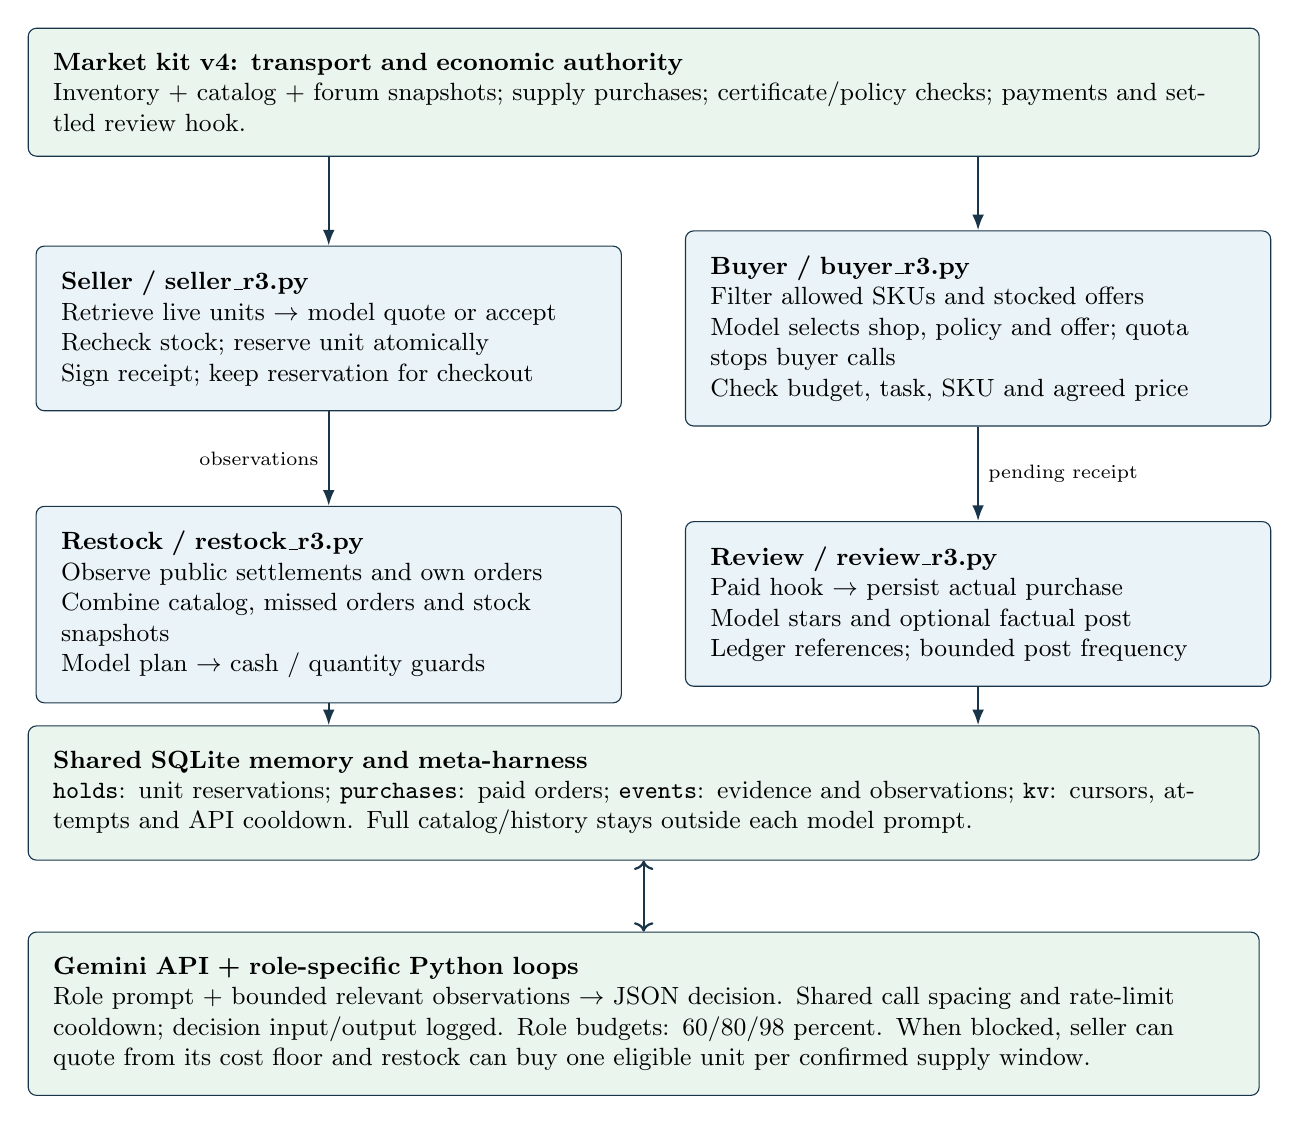
\begin{tikzpicture}[
 node distance=9mm and 8mm,
 box/.style={draw=ink,rounded corners=3pt,fill=pale,text width=68mm,align=left,inner sep=9pt,font=\small},
 state/.style={box,fill=green,text width=150mm},
 arr/.style={-{Latex[length=2mm]},thick,draw=ink}]
\node[state] (kit) {\textbf{Market kit v4: transport and economic authority}\\Inventory + catalog + forum snapshots; supply purchases; certificate/policy checks; payments and settled review hook.};
\node[box] (seller) at (-4,-3) {\textbf{Seller / seller\_r3.py}\\Retrieve live units $\rightarrow$ model quote or accept\\Recheck stock; reserve unit atomically\\Sign receipt; keep reservation for checkout};
\node[box,right=8mm of seller] (buyer) {\textbf{Buyer / buyer\_r3.py}\\Filter allowed SKUs and stocked offers\\Model selects shop, policy and offer; quota stops buyer calls\\Check budget, task, SKU and agreed price};
\draw[arr] (kit.south -| seller.north) -- (seller.north);
\draw[arr] (kit.south -| buyer.north) -- (buyer.north);
\node[box,below=12mm of seller] (restock) {\textbf{Restock / restock\_r3.py}\\Observe public settlements and own orders\\Combine catalog, missed orders and stock snapshots\\Model plan $\rightarrow$ cash / quantity guards};
\node[box,below=12mm of buyer] (review) {\textbf{Review / review\_r3.py}\\Paid hook $\rightarrow$ persist actual purchase\\Model stars and optional factual post\\Ledger references; bounded post frequency};
\draw[arr] (seller) -- node[left,font=\scriptsize]{observations} (restock);
\draw[arr] (buyer) -- node[right,font=\scriptsize]{pending receipt} (review);
\node[state] (memory) at (0,-8.9) {\textbf{Shared SQLite memory and meta-harness}\\\texttt{holds}: unit reservations; \texttt{purchases}: paid orders; \texttt{events}: evidence and observations; \texttt{kv}: cursors, attempts and API cooldown. Full catalog/history stays outside each model prompt.};
\draw[arr] (restock.south) -- (restock.south |- memory.north);
\draw[arr] (review.south) -- (review.south |- memory.north);
\node[state,below=9mm of memory] (model) {\textbf{Gemini API + role-specific Python loops}\\Role prompt + bounded relevant observations $\rightarrow$ JSON decision. Shared call spacing and rate-limit cooldown; decision input/output logged. Role budgets: 60/80/98 percent. When blocked, seller can quote from its cost floor and restock can buy one eligible unit per confirmed supply window.};
\draw[arr,<->] (memory) -- (model);
\end{tikzpicture}
\end{center}
\vspace{6pt}
\noindent\textbf{External communication.} Buyer negotiates with other sellers over A2A 1.0 JSON-RPC. The kit executes supply, payment and forum operations; the diagram's local buyer and seller do not trade with each other.\\[8pt]
\noindent\textbf{Boundaries and limitations.} Retrieval limits introduce selection bias. Initial reviews cannot know later failures. Ambiguous same-name breakage is not assigned to one shop. A failed checkout is not automatically renegotiated. Use ACP records to distinguish pending receipts from completed payments. Evaluate fallback outcomes in a separate live run.
\end{document}
